\section{Attributes}

An attribute is a specific detail about a node. Attributes are used by the chef-client to understand:

\begin{itemize}
  \item The current state of the node
  \item What the state of the node was at the end of the previous chef-client run
  \item What the state of the node should be at the end of the current chef-client run
\end{itemize}

As you read from previous sections of book, attributes can be defined in node, roles and environments, but it's also can be defined by cookbooks.

\subsection{Attribute Types}

Attribute types can be any of the following:

\begin{itemize}
  \item \textbf{default} - attribute is automatically reset at the start of every chef-client run and has the lowest attribute precedence
  \item \textbf{force\_default} - attribute is used to ensure that an attribute defined in a cookbook (by an attribute file or by a recipe) takes precedence over a default attribute set by a role or an environment
  \item \textbf{normal} - attribute is a setting that persists on the target system and is never reset during a chef-client run. A normal attribute has a higher attribute precedence than a default attribute
  \item \textbf{override} - attribute is automatically reset at the start of every chef-client run and has a higher attribute precedence than default, force\_default, and normal attributes. An override attribute is most often specified in a recipe, but can be specified in an attribute file, for a role, and/or for an environment
  \item \textbf{force\_override} - attribute is used to ensure that an attribute defined in a cookbook (by an attribute file or by a recipe) takes precedence over an override attribute set by a role or an environment
  \item \textbf{automatic} - attribute contains data that is identified by Ohai at the beginning of every chef-client run. An automatic attribute cannot be modified and always has the highest attribute precedence
\end{itemize}

At the beginning of a chef-client run, all default, override, and automatic attributes are reset. The chef-client rebuilds them using data collected by Ohai at the beginning of the chef-client run and by attributes that are defined in cookbooks, roles, and environments. Normal attributes are never reset. All attributes are then merged and applied to the node according to attribute precedence. At the conclusion of the chef-client run, all default, override, and automatic attributes disappear, leaving only a collection of normal attributes that will persist until the next chef-client run.

\subsection{Automatic (Ohai)}

An automatic attribute is a specific detail about a node, such as an IP address, a host name, a list of loaded kernel modules, and so on. Automatic attributes are detected by Ohai and are then used by the chef-client to ensure that these attribute are handled properly during every chef-client run. The most commonly accessed automatic attributes are:

\begin{itemize}
  \item \textbf{node['platform']} - the platform on which a node is running. This attribute helps determine which providers will be used
  \item \textbf{node['platform\_version']} - the version of the platform. This attribute helps determine which providers will be used
  \item \textbf{node['ipaddress']} - the IP address for a node. If the node has a default route, this is the IPV4 address for the interface. If the node does not have a default route, the value for this attribute should be nil. The IP address for default route is the recommended default value
  \item \textbf{node['macaddress']} - the MAC address for a node, determined by the same interface that detects the <<node['ipaddress']>>
  \item \textbf{node['fqdn']} - the fully qualified domain name for a node. This is used as the name of a node unless otherwise set
  \item \textbf{node['hostname']} - the host name for the nod
  \item \textbf{node['domain']} - the domain for the node
  \item \textbf{node['recipes']} - a list of recipes associated with a node (and part of that node’s run-list)
  \item \textbf{node['roles']} - a list of roles associated with a node (and part of that node’s run-list)
\end{itemize}

The list of automatic attributes that are collected by Ohai at the start of each chef-client run vary from organization to organization, and will often vary between the various server types being configured and the platforms on which those servers are run. All attributes collected by Ohai are unmodifiable by the chef-client.

\subsection{Attribute Precedence}

Attribute types can be any of the following:

\begin{enumerate}
  \item A \textbf{default} attribute located in a cookbook attribute file
  \item A \textbf{default} attribute located in a recipe
  \item A \textbf{default} attribute located in an environment
  \item A \textbf{default} attribute located in role
  \item A \textbf{force\_default} attribute located in a cookbook attribute file
  \item A \textbf{force\_default} attribute located in a recipe
  \item A \textbf{normal} attribute located in a cookbook attribute file
  \item A \textbf{normal} attribute located in a recipe
  \item An \textbf{override} attribute located in a cookbook attribute file
  \item An \textbf{override} attribute located in a recipe
  \item An \textbf{override} attribute located in a role
  \item An \textbf{override} attribute located in an environment
  \item A \textbf{force\_override} attribute located in a cookbook attribute file
  \item A \textbf{force\_override} attribute located in a recipe
  \item An \textbf{automatic} attribute identified by Ohai at the start of the chef-client run
\end{enumerate}

where the last attribute in the list is the one that is applied to the node.

Attribute precedence, viewed from the same perspective as the overview diagram~\ref{fig:overview_chef_attributes_precedence}, where the numbers in the diagram match the order of attribute precedence:

\begin{figure}[ht!]
  \center{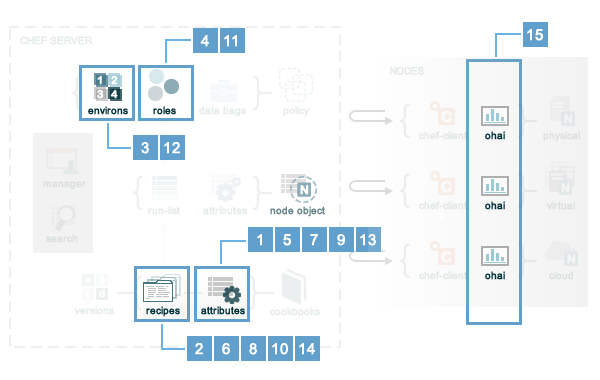
\includegraphics[width=1\textwidth]{overview_chef_attributes_precedence}}
  \caption{Attribute precedence}
  \label{fig:overview_chef_attributes_precedence}
\end{figure}

Attribute precedence~\ref{fig:overview_chef_attributes_table}, when viewed as a table:

\begin{figure}[ht!]
  \center{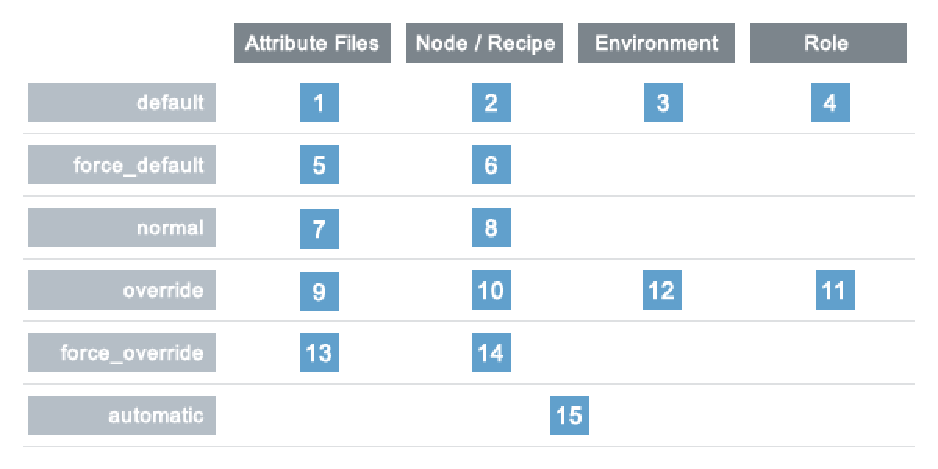
\includegraphics[width=1\textwidth]{overview_chef_attributes_table}}
  \caption{Attribute precedence}
  \label{fig:overview_chef_attributes_table}
\end{figure}